% ========================================================
% VERIFICACIÓN FORMAL EN SPIN (ENTREGABLE 3)
% ========================================================
% Los rangos de líneas de kmeans.pml que se citan abajo: si el modelo cambia, `make informe`
% en tp/spin/ falla hasta que se actualicen (comprueba que la línea 113 sea la barrera).
\section{Verificación formal en Spin: deadlock, exclusión mutua y progreso}\label{sec:verificacion}

El enunciado del Entregable 3 pide verificar formalmente dos propiedades del algoritmo: que no tiene
\emph{deadlocks} y que respeta la exclusión mutua. La Sección~\ref{sec:promela} ya las comprobaba con
aserciones sobre el modelo de la PC2. Este entregable las expresa además como fórmulas de lógica
temporal lineal (LTL), agrega una tercera, la de progreso, y sobre todo demuestra que cada
verificación es capaz de fallar: para cada propiedad hay un mutante del modelo que la viola, y Spin
tiene que encontrar ese error y no otro.

\subsection{Las tres propiedades}

\paragraph{Ausencia de deadlock.} En Spin, un deadlock es un \emph{estado final inválido}: la
búsqueda llega a un estado desde el que ningún proceso puede avanzar, y al menos uno quedó bloqueado
en un punto que no lleva la etiqueta \texttt{end}. Los workers que esperan trabajo en
\texttt{trabajos ? idx} están bajo \texttt{end:}, que declara legítima esa espera: es lo que hace
un worker del pool entre iteraciones. Si la barrera nunca llega a cero, el proceso que queda
bloqueado es \texttt{init}, en la guarda \texttt{pendientes == 0}, y \texttt{pan} lo reporta.
Esta propiedad no necesita fórmula: \texttt{pan} la comprueba por su cuenta en cada búsqueda de
seguridad.

\paragraph{Exclusión mutua.} El recurso compartido son los centroides. Los lectores son los workers
mientras asignan viajes, contados en \texttt{lectores}; el escritor es el coordinador mientras
publica los centroides nuevos, con \texttt{escribiendo = 1}. La propiedad exige que las dos cosas no
ocurran nunca a la vez, en ningún entrelazado:
\[
  \textit{exclusion} \;=\; \Box\, \neg\,(\textit{escribiendo} \wedge \textit{lectores} > 0).
\]

\paragraph{Progreso.} Que no haya deadlock no garantiza que la corrida termine: el sistema podría
avanzar para siempre sin llegar al final. La propiedad de progreso es que las dos iteraciones
terminan, $\textit{termina} = \Diamond\, \textit{fin}$, donde \texttt{fin} se activa al salir del
lazo de iteraciones. Una propiedad así solo vale bajo una hipótesis sobre el planificador. Se usa
\emph{weak fairness} (\texttt{pan -a -f}): ningún proceso que queda habilitado para siempre se
posterga para siempre. Es la hipótesis que da el planificador de Go para una goroutine ejecutable, y
es más débil que suponer un orden particular de ejecución.

El Listado~\ref{lst:ltl} muestra las dos fórmulas tal como están en el modelo.

\needspace{10\baselineskip}
\lstinputlisting[language=Promela, firstline=134, lastline=139, firstnumber=134,
                 caption={Fórmulas LTL de \texttt{tp/spin/kmeans.pml}}, label={lst:ltl}]
                {../../spin/kmeans.pml}

\subsection{Un mutante por propiedad}

Que \texttt{pan} responda \texttt{errors: 0} solo convence si el mismo chequeo responde
\texttt{errors: 1} cuando el algoritmo está mal. Por eso cada propiedad tiene una variante del
modelo que la rompe, con el error más probable en la implementación real. Las variantes son el
mismo archivo compilado con un \texttt{-D} distinto, de modo que la diferencia con el modelo correcto
es exactamente la línea que cambia.

\paragraph{\texttt{MUTANTE\_DEADLOCK}: un \texttt{wg.Done} perdido.} El worker que procesa el
último bloque no decrementa \texttt{pendientes} (Listado~\ref{lst:mut-deadlock}). En Go es el error
típico de un \texttt{return} temprano antes del \texttt{wg.Done()}, o de un \texttt{Done} que no está
en un \texttt{defer}. La barrera queda esperando un bloque que ya se procesó.

\needspace{13\baselineskip}
\lstinputlisting[language=Promela, firstline=80, lastline=88, firstnumber=80,
                 caption={El \texttt{wg.Done} condicional del mutante de deadlock},
                 label={lst:mut-deadlock}]{../../spin/kmeans.pml}

\paragraph{\texttt{MUTANTE\_SIN\_BARRERA}: publicar sin esperar.} El coordinador se salta la
barrera y el \texttt{assert(lectores == 0)} que la acompaña (Listado~\ref{lst:barrera}), y publica
los centroides nuevos apenas termina de encolar los bloques. En Go equivale a llamar a
\texttt{actualizar} sin \texttt{wg.Wait()}. El \texttt{assert} se salta también porque, si quedara,
detectaría el error antes que la fórmula, y lo que se quiere probar es que la fórmula lo detecta.

\needspace{15\baselineskip}
\lstinputlisting[language=Promela, firstline=107, lastline=117, firstnumber=107,
                 caption={La barrera del coordinador, que el mutante sin barrera omite},
                 label={lst:barrera}]{../../spin/kmeans.pml}

El tercer mutante es el de la PC2, \texttt{MUTANTE}: el acumulador compartido sin exclusión mutua
de la Sección~\ref{sec:promela}.

\subsection{Resultados}

La Tabla~\ref{tab:spin-casos} resume los siete casos. Cada fila es una corrida de \texttt{pan} con
búsqueda exhaustiva sobre SPIN 6.5.2; la tabla se genera desde la salida de la regresión
(\texttt{make informe} en \texttt{tp/spin/}), sin transcribir cifras. La
Figura~\ref{fig:ejec-spin-check} es la ejecución de esa regresión: cada caso compara el número de
errores contra el esperado.

\begin{figure}[tbp]
\caption{Ejecución de la regresión de Spin: los siete casos}\label{fig:ejec-spin-check}
\centering
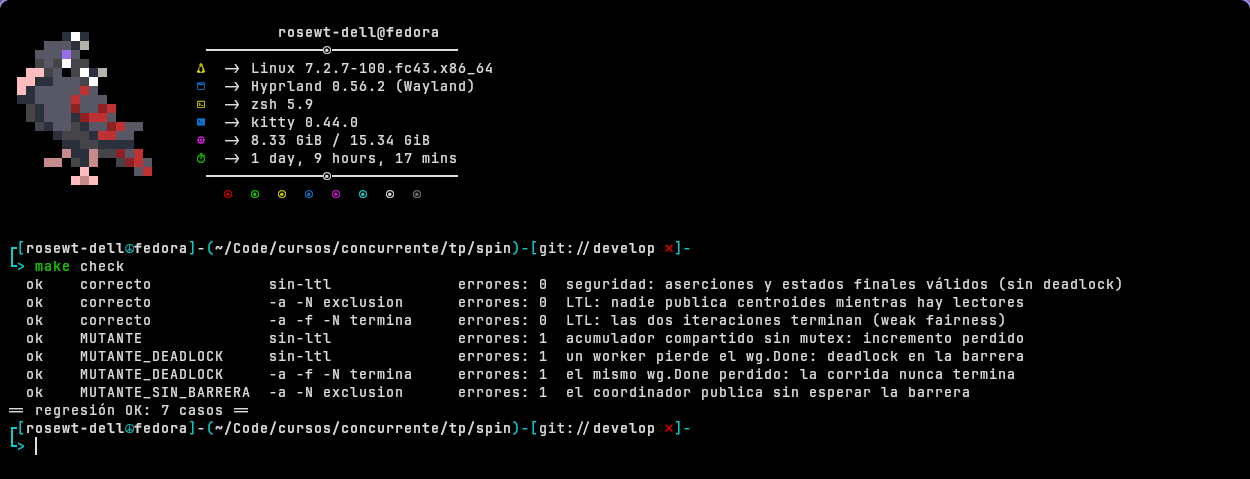
\includegraphics[width=\textwidth,height=0.72\textheight,keepaspectratio]{img/ejec-spin-check.png}
\end{figure}

\begin{table}[H]
\caption{Verificación del modelo correcto y de los tres mutantes}\label{tab:spin-casos}
\small
% Generado por tp/scripts/figuras_spin.py desde spin-casos.tsv (make informe). No editar.
\begin{tabularx}{\textwidth}{@{}L{4.1cm}L{3.1cm}rrrY@{}}
\toprule
\textbf{Variante} & \textbf{Corrida de \texttt{pan}} & \textbf{Err.} & \textbf{Estados} & \textbf{Prof.} & \textbf{Resultado} \\
\midrule
correcto & seguridad (\texttt{-DNOCLAIM}) & 0 & 2\,412 & 181 & sin errores \\
\multicolumn{6}{@{}l}{\footnotesize\textit{seguridad: aserciones y estados finales válidos (sin deadlock)}} \\
\addlinespace
correcto & \texttt{-a -N exclusion} & 0 & 2\,412 & 362 & sin errores \\
\multicolumn{6}{@{}l}{\footnotesize\textit{LTL: nadie publica centroides mientras hay lectores}} \\
\addlinespace
correcto & \texttt{-a -f -N termina} & 0 & 2\,412 & 361 & sin errores \\
\multicolumn{6}{@{}l}{\footnotesize\textit{LTL: las dos iteraciones terminan (weak fairness)}} \\
\addlinespace
\texttt{MUTANTE} & seguridad (\texttt{-DNOCLAIM}) & 1 & 393 & 209 & \texttt{assertion violated (compartido==4)} \\
\multicolumn{6}{@{}l}{\footnotesize\textit{acumulador compartido sin mutex: incremento perdido}} \\
\addlinespace
\texttt{MUTANTE\_DEADLOCK} & seguridad (\texttt{-DNOCLAIM}) & 1 & 65 & 65 & \texttt{invalid end state} \\
\multicolumn{6}{@{}l}{\footnotesize\textit{un worker pierde el wg.Done: deadlock en la barrera}} \\
\addlinespace
\texttt{MUTANTE\_DEADLOCK} & \texttt{-a -f -N termina} & 1 & 65 & 132 & \texttt{acceptance cycle} \\
\multicolumn{6}{@{}l}{\footnotesize\textit{el mismo wg.Done perdido: la corrida nunca termina}} \\
\addlinespace
\texttt{MUTANTE\_SIN\_BARRERA} & \texttt{-a -N exclusion} & 1 & 206 & 354 & viola la fórmula \texttt{exclusion} \\
\multicolumn{6}{@{}l}{\footnotesize\textit{el coordinador publica sin esperar la barrera}} \\
\bottomrule
\end{tabularx}


\smallskip
{\footnotesize\textit{Nota.} «Seguridad» es la búsqueda de violaciones de aserciones y de estados
finales inválidos, compilada con \texttt{-DNOCLAIM}. \texttt{-a} busca ciclos de aceptación de la
fórmula nombrada con \texttt{-N}; \texttt{-f} agrega weak fairness. «Prof.» es la profundidad
máxima alcanzada. Las búsquedas que encuentran un error se detienen en el primero, por eso visitan
menos estados.\par}
\end{table}

\paragraph{El modelo correcto cumple las tres propiedades.} Las tres búsquedas recorren los mismos
2\,412 estados y terminan sin errores. La de progreso es la más costosa, porque con fairness
\texttt{pan} explora el producto del modelo con el autómata de la fórmula
(Figura~\ref{fig:spin-termina}).

\needspace{21\baselineskip}
\begin{figure}[tbp]
\caption{Ejecución de \texttt{pan -a -f -N termina} sobre el modelo correcto}\label{fig:spin-termina}
\centering
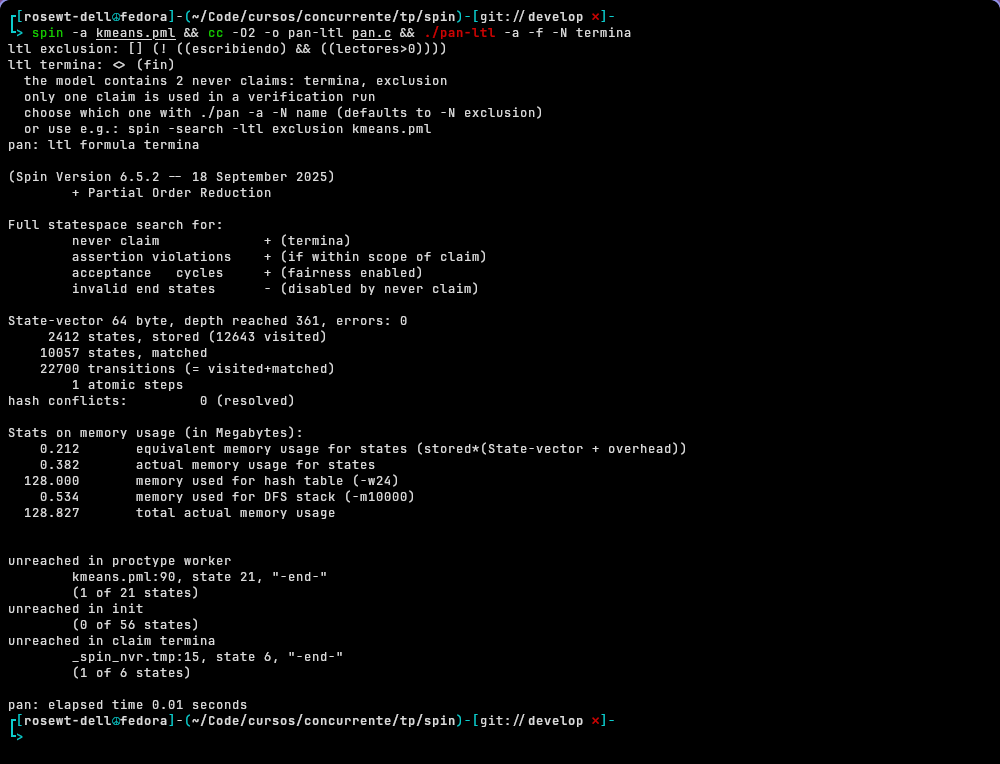
\includegraphics[width=\textwidth,height=0.72\textheight,keepaspectratio]{img/ejec-spin-termina.png}
\end{figure}

\paragraph{El deadlock aparece en la primera iteración.} Con el \texttt{wg.Done} perdido, Spin
encuentra un estado final inválido a profundidad 64. La Figura~\ref{fig:traza-deadlock} es el
estado del sistema al final del contraejemplo, reproducido con \texttt{spin -t}: los cuatro puntos
fueron procesados (\texttt{seen[i] = 1}), los dos bloques tienen sus dos puntos
(\texttt{conteo[c] = 2}), pero \texttt{pendientes} quedó en 1. Los dos workers están en la línea 61,
esperando trabajo en un canal vacío, que es un estado final válido, e \texttt{init} está bloqueado
en la línea 113, la guarda \texttt{pendientes == 0}, que no lo es. Nadie puede avanzar. Todo el
trabajo se hizo y el programa no termina: es exactamente el síntoma de un \texttt{wg.Done} perdido.

\needspace{30\baselineskip}
\begin{figure}[tbp]
\caption{Estado final del contraejemplo de \texttt{MUTANTE\_DEADLOCK} (\texttt{spin -t -g -l -p})}\label{fig:traza-deadlock}
\centering
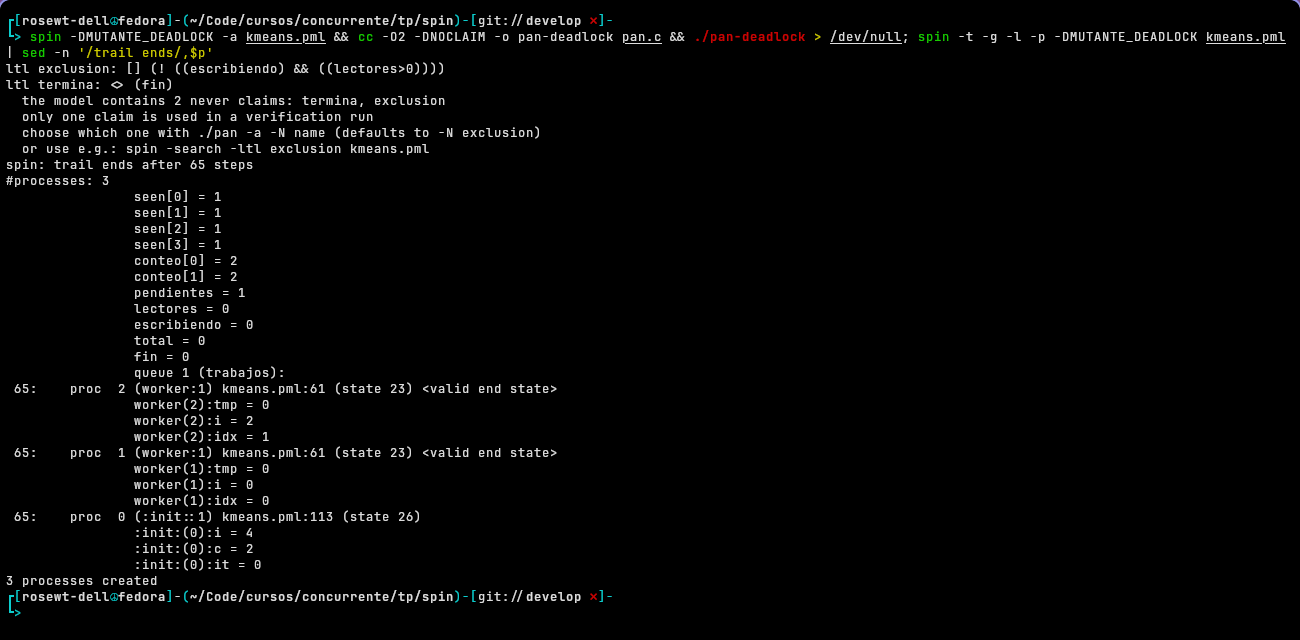
\includegraphics[width=\textwidth,height=0.72\textheight,keepaspectratio]{img/ejec-traza-deadlock.png}
\end{figure}

El mismo mutante viola también la fórmula de progreso: \texttt{pan -a -f -N termina} encuentra un
ciclo de aceptación, una ejecución infinita en la que \texttt{fin} no se activa nunca. Las dos
búsquedas encuentran el mismo error desde dos lados: la de seguridad ve el estado bloqueado, la de
progreso ve que la corrida no llega a su final.

\paragraph{Sin barrera se publica con lectores.} Con el coordinador que no espera, la fórmula
\texttt{exclusion} se viola a profundidad 295: hay un entrelazado en el que un worker todavía está
leyendo los centroides cuando el coordinador empieza a escribirlos. Es la carrera que la barrera
evita, y es la razón por la que el Algoritmo~\ref{alg:lloyd-chunks} sincroniza antes de reducir y no
después.

\subsection{Tres trampas de \texttt{pan}}

Tres veces, al construir la regresión, \texttt{pan} dio un resultado falso sin avisar. Las tres
quedaron cubiertas en \texttt{tp/spin/check.sh}.

\begin{itemize}
  \item \textbf{Con fórmulas en el archivo, \texttt{pan} deja de buscar deadlocks.} Sin \texttt{-N},
        usa la primera fórmula como \emph{never claim} y desactiva la búsqueda de estados finales
        inválidos: su salida dice \texttt{invalid end states - (disabled by never claim)}. La corrida
        de seguridad dejaba de encontrar el deadlock del mutante. La opción \texttt{-noclaim} que
        parecía resolverlo no existe y se ignora en silencio. Lo que funciona es compilar con
        \texttt{-DNOCLAIM}, y la regresión exige que la salida diga \texttt{invalid end states +}.
  \item \textbf{\texttt{-N} con un nombre que no existe no verifica nada.} Da \texttt{errors: 0},
        como un modelo correcto. Pasó al escribir la regresión antes que las fórmulas: los casos del
        modelo correcto «pasaban». Ahora la regresión exige que la fórmula figure en la salida como
        el never claim activo.
  \item \textbf{\texttt{-A} también apaga la fórmula.} Spin traduce una fórmula de seguridad
        $\Box p$ a un never claim con un \texttt{assert} adentro, y \texttt{-A}, que desactiva las
        aserciones, desactiva también ese. Por eso no se usa, y el tipo de error esperado para el
        mutante sin barrera nombra la fórmula y no cualquier aserción.
\end{itemize}

La lección general es la misma del mutante de la PC2, un nivel más arriba: no alcanza con que la
herramienta responda, hay que comprobar que respondió la pregunta que se le hizo. Por eso la
regresión exige, para cada caso, el número de errores y además el tipo de error, y corre en la
integración continua de GitHub con cada cambio en \texttt{tp/spin/}.

\subsection{Relación con la implementación y límites}

El deadlock del mutante tiene un equivalente directo en Go: si una goroutine del pool se salta el
\texttt{wg.Done()}, \texttt{wg.Wait()} no retorna nunca. El runtime de Go detecta ese caso solo
cuando \emph{todas} las goroutines quedan bloqueadas y termina con \texttt{all goroutines are asleep
- deadlock!}; en un programa con otras goroutines activas, como un servidor, se queda colgado sin
aviso. Un test lo encuentra solo si ejecuta el camino que pierde el \texttt{Done}. Spin lo encuentra
en el diseño, sobre todos los entrelazados, antes de que exista ese camino en el código. En la
implementación, el \texttt{Done} de cada bloque se llama incondicionalmente al terminarlo, que es la
forma de evitar el error que el mutante introduce.

Los límites son los de la Sección~\ref{sec:promela}: cuatro puntos, dos bloques, dos workers y dos
iteraciones. El progreso vale bajo weak fairness, no para cualquier planificador. El cierre del pool,
\texttt{close(trabajos)} seguido de esperar a que las goroutines terminen, no está modelado: en el
modelo los workers terminan bloqueados en el canal, lo que \texttt{end:} declara legítimo. Verificar
ese cierre requeriría modelar el cierre del canal y agregar una propiedad de terminación de los
workers.
